\documentclass[a4paper]{book}
\usepackage{a4wide}
\usepackage{makeidx}
\usepackage{graphicx}
\usepackage{multicol}
\usepackage{float}
\usepackage{listings}
\usepackage{color}
\usepackage{textcomp}
\usepackage{alltt}
\usepackage{times}
\usepackage{ifpdf}
\ifpdf
\usepackage[pdftex,
            pagebackref=true,
            colorlinks=true,
            linkcolor=blue,
            unicode
           ]{hyperref}
\else
\usepackage[ps2pdf,
            pagebackref=true,
            colorlinks=true,
            linkcolor=blue,
            unicode
           ]{hyperref}
\usepackage{pspicture}
\fi
\usepackage[utf8]{inputenc}
\usepackage{doxygen}
\lstset{language=C++,inputencoding=utf8,basicstyle=\footnotesize,breaklines=true,breakatwhitespace=true,tabsize=8,numbers=left }
\makeindex
\setcounter{tocdepth}{3}
\renewcommand{\footrulewidth}{0.4pt}
\begin{document}
\hypersetup{pageanchor=false}
\begin{titlepage}
\vspace*{7cm}
\begin{center}
{\Large Reference Manual}\\
\vspace*{1cm}
{\large Generated by Doxygen 1.6.3}\\
\vspace*{0.5cm}
{\small Mon Feb 28 13:44:44 2011}\\
\end{center}
\end{titlepage}
\clearemptydoublepage
\pagenumbering{roman}
\tableofcontents
\clearemptydoublepage
\pagenumbering{arabic}
\hypersetup{pageanchor=true}
\chapter{Class Index}
\section{Class Hierarchy}
This inheritance list is sorted roughly, but not completely, alphabetically:\begin{DoxyCompactList}
\item \contentsline{section}{\_\-Bot}{\pageref{struct__Bot}}{}
\item \contentsline{section}{\_\-Frame}{\pageref{struct__Frame}}{}
\item \contentsline{section}{\_\-Mappable}{\pageref{struct__Mappable}}{}
\item \contentsline{section}{\_\-Type}{\pageref{struct__Type}}{}
\item \contentsline{section}{\_\-Unit}{\pageref{struct__Unit}}{}
\item \contentsline{section}{\_\-Wall}{\pageref{struct__Wall}}{}
\item \contentsline{section}{BaseAI}{\pageref{classBaseAI}}{}
\begin{DoxyCompactList}
\item \contentsline{section}{AI}{\pageref{classAI}}{}
\end{DoxyCompactList}
\item \contentsline{section}{Connection}{\pageref{structConnection}}{}
\item \contentsline{section}{Mappable}{\pageref{classMappable}}{}
\begin{DoxyCompactList}
\item \contentsline{section}{Unit}{\pageref{classUnit}}{}
\begin{DoxyCompactList}
\item \contentsline{section}{Bot}{\pageref{classBot}}{}
\item \contentsline{section}{Frame}{\pageref{classFrame}}{}
\item \contentsline{section}{Wall}{\pageref{classWall}}{}
\end{DoxyCompactList}
\end{DoxyCompactList}
\item \contentsline{section}{Type}{\pageref{classType}}{}
\end{DoxyCompactList}

\chapter{Class Index}
\section{Class List}
Here are the classes, structs, unions and interfaces with brief descriptions:\begin{DoxyCompactList}
\item\contentsline{section}{\hyperlink{classAI_1_1AI}{AI::AI} }{\pageref{classAI_1_1AI}}{}
\item\contentsline{section}{\hyperlink{classBaseAI_1_1BaseAI}{BaseAI::BaseAI} }{\pageref{classBaseAI_1_1BaseAI}}{}
\item\contentsline{section}{\hyperlink{classGameObject_1_1Bot}{GameObject::Bot} (The bot class )}{\pageref{classGameObject_1_1Bot}}{}
\item\contentsline{section}{\hyperlink{classExistentialError_1_1ExistentialError}{ExistentialError::ExistentialError} }{\pageref{classExistentialError_1_1ExistentialError}}{}
\item\contentsline{section}{\hyperlink{classGameObject_1_1Frame}{GameObject::Frame} (A baby robot )}{\pageref{classGameObject_1_1Frame}}{}
\item\contentsline{section}{\hyperlink{classGameObject_1_1GameObject}{GameObject::GameObject} }{\pageref{classGameObject_1_1GameObject}}{}
\item\contentsline{section}{\hyperlink{classGameObject_1_1Mappable}{GameObject::Mappable} (An object that exists on the grid )}{\pageref{classGameObject_1_1Mappable}}{}
\item\contentsline{section}{\hyperlink{classGameObject_1_1Type}{GameObject::Type} (A kind of robot )}{\pageref{classGameObject_1_1Type}}{}
\item\contentsline{section}{\hyperlink{classGameObject_1_1Unit}{GameObject::Unit} (An object that exists on the grid )}{\pageref{classGameObject_1_1Unit}}{}
\item\contentsline{section}{\hyperlink{classGameObject_1_1Wall}{GameObject::Wall} (A pile of hard stuff that is in the way )}{\pageref{classGameObject_1_1Wall}}{}
\end{DoxyCompactList}

\chapter{Class Documentation}
\hypertarget{struct__Bot}{
\section{\_\-Bot Struct Reference}
\label{struct__Bot}\index{\_\-Bot@{\_\-Bot}}
}
\subsection*{Public Attributes}
\begin{DoxyCompactItemize}
\item 
\hypertarget{struct__Bot_a8eace064ca320a504ebd4346a46e24ba}{
\hyperlink{structConnection}{Connection} $\ast$ {\bfseries \_\-c}}
\label{struct__Bot_a8eace064ca320a504ebd4346a46e24ba}

\item 
\hypertarget{struct__Bot_a210750792cc706e75346904a1e4fcba9}{
int {\bfseries id}}
\label{struct__Bot_a210750792cc706e75346904a1e4fcba9}

\item 
\hypertarget{struct__Bot_a4f57cab815e10b59bd35fd22eb6c4ae0}{
int {\bfseries x}}
\label{struct__Bot_a4f57cab815e10b59bd35fd22eb6c4ae0}

\item 
\hypertarget{struct__Bot_af97ef8695aee6f7de31a5b3e9e5efede}{
int {\bfseries y}}
\label{struct__Bot_af97ef8695aee6f7de31a5b3e9e5efede}

\item 
\hypertarget{struct__Bot_ac9e9133a82f52ac8feeb21ef50378ae1}{
int {\bfseries owner}}
\label{struct__Bot_ac9e9133a82f52ac8feeb21ef50378ae1}

\item 
\hypertarget{struct__Bot_a2daffc482e65fd50c8e405b416ad7691}{
int {\bfseries health}}
\label{struct__Bot_a2daffc482e65fd50c8e405b416ad7691}

\item 
\hypertarget{struct__Bot_ad0b78f544be40a0ce920c1be6418528e}{
int {\bfseries maxHealth}}
\label{struct__Bot_ad0b78f544be40a0ce920c1be6418528e}

\item 
\hypertarget{struct__Bot_ac536a158e666e25c3616337ca3200720}{
int {\bfseries size}}
\label{struct__Bot_ac536a158e666e25c3616337ca3200720}

\item 
\hypertarget{struct__Bot_a8e5e38855bd71b564f5f549474601c02}{
int {\bfseries actions}}
\label{struct__Bot_a8e5e38855bd71b564f5f549474601c02}

\item 
\hypertarget{struct__Bot_a448ebaed89622ad99f34c1aedd0238dc}{
int {\bfseries steps}}
\label{struct__Bot_a448ebaed89622ad99f34c1aedd0238dc}

\item 
\hypertarget{struct__Bot_a869d2150e92439a163792581bcae0af2}{
int {\bfseries damage}}
\label{struct__Bot_a869d2150e92439a163792581bcae0af2}

\item 
\hypertarget{struct__Bot_af77000f12da1b214a6e8eba86994d1bf}{
int {\bfseries range}}
\label{struct__Bot_af77000f12da1b214a6e8eba86994d1bf}

\item 
\hypertarget{struct__Bot_a2dc620ec845ee001bc90609df5a5ce1f}{
int {\bfseries movitude}}
\label{struct__Bot_a2dc620ec845ee001bc90609df5a5ce1f}

\item 
\hypertarget{struct__Bot_a92ea66d0f290429aa732b28a872e23c7}{
int {\bfseries actitude}}
\label{struct__Bot_a92ea66d0f290429aa732b28a872e23c7}

\item 
\hypertarget{struct__Bot_ac81d97c9fc26363210eb3e6e8736fdf3}{
int {\bfseries buildRate}}
\label{struct__Bot_ac81d97c9fc26363210eb3e6e8736fdf3}

\item 
\hypertarget{struct__Bot_ae03ba29225a1468b981bc44faf0aabed}{
int {\bfseries partOf}}
\label{struct__Bot_ae03ba29225a1468b981bc44faf0aabed}

\item 
\hypertarget{struct__Bot_a7784a3b6301ea5d3556ab5ef93fb4dc7}{
int {\bfseries building}}
\label{struct__Bot_a7784a3b6301ea5d3556ab5ef93fb4dc7}

\item 
\hypertarget{struct__Bot_a460e784b7657c229eccea105479268cd}{
int {\bfseries type}}
\label{struct__Bot_a460e784b7657c229eccea105479268cd}

\end{DoxyCompactItemize}


The documentation for this struct was generated from the following file:\begin{DoxyCompactItemize}
\item 
structures.h\end{DoxyCompactItemize}

\hypertarget{struct__Frame}{
\section{\_\-Frame Struct Reference}
\label{struct__Frame}\index{\_\-Frame@{\_\-Frame}}
}
\subsection*{Public Attributes}
\begin{DoxyCompactItemize}
\item 
\hypertarget{struct__Frame_a85d8d05ce9f31edc328c1bf12f1aaccd}{
\hyperlink{structConnection}{Connection} $\ast$ {\bfseries \_\-c}}
\label{struct__Frame_a85d8d05ce9f31edc328c1bf12f1aaccd}

\item 
\hypertarget{struct__Frame_a625f3af04536d2e0f493c05fac69846a}{
int {\bfseries id}}
\label{struct__Frame_a625f3af04536d2e0f493c05fac69846a}

\item 
\hypertarget{struct__Frame_ac14551c123b762ce73d9a616f5c91195}{
int {\bfseries x}}
\label{struct__Frame_ac14551c123b762ce73d9a616f5c91195}

\item 
\hypertarget{struct__Frame_a32484dd5600487febf8c3585ad85ff56}{
int {\bfseries y}}
\label{struct__Frame_a32484dd5600487febf8c3585ad85ff56}

\item 
\hypertarget{struct__Frame_a2d16e0cb9efa4fe4e5ce5d65db47bfa5}{
int {\bfseries owner}}
\label{struct__Frame_a2d16e0cb9efa4fe4e5ce5d65db47bfa5}

\item 
\hypertarget{struct__Frame_ae72a3ac0ec1416c7902faf59e8a4047e}{
int {\bfseries health}}
\label{struct__Frame_ae72a3ac0ec1416c7902faf59e8a4047e}

\item 
\hypertarget{struct__Frame_a86d50983f8ff48141bde8859bdf09b42}{
int {\bfseries maxHealth}}
\label{struct__Frame_a86d50983f8ff48141bde8859bdf09b42}

\item 
\hypertarget{struct__Frame_a5b892f0794b3fe35e65708e3a03e4985}{
int {\bfseries size}}
\label{struct__Frame_a5b892f0794b3fe35e65708e3a03e4985}

\item 
\hypertarget{struct__Frame_a80a067fe44266acfb51000098e58d797}{
\hyperlink{struct__Type}{\_\-Type} $\ast$ {\bfseries type}}
\label{struct__Frame_a80a067fe44266acfb51000098e58d797}

\item 
\hypertarget{struct__Frame_adfad76a0dd5a9621664c3f2622ee2c6b}{
int {\bfseries completionTime}}
\label{struct__Frame_adfad76a0dd5a9621664c3f2622ee2c6b}

\end{DoxyCompactItemize}


The documentation for this struct was generated from the following file:\begin{DoxyCompactItemize}
\item 
structures.h\end{DoxyCompactItemize}

\hypertarget{struct__Mappable}{
\section{\_\-Mappable Struct Reference}
\label{struct__Mappable}\index{\_\-Mappable@{\_\-Mappable}}
}
\subsection*{Public Attributes}
\begin{DoxyCompactItemize}
\item 
\hypertarget{struct__Mappable_a7ec82fd98d694fbdbb8c61f9d43f1b5b}{
\hyperlink{structConnection}{Connection} $\ast$ {\bfseries \_\-c}}
\label{struct__Mappable_a7ec82fd98d694fbdbb8c61f9d43f1b5b}

\item 
\hypertarget{struct__Mappable_aad5451cf1ea111ea63c72fbeedeef1cc}{
int {\bfseries id}}
\label{struct__Mappable_aad5451cf1ea111ea63c72fbeedeef1cc}

\item 
\hypertarget{struct__Mappable_a99b450814ecd057e5f0dd7f47f443e8e}{
int {\bfseries x}}
\label{struct__Mappable_a99b450814ecd057e5f0dd7f47f443e8e}

\item 
\hypertarget{struct__Mappable_a941d0fc2565e112b4e05b2a40f65f30f}{
int {\bfseries y}}
\label{struct__Mappable_a941d0fc2565e112b4e05b2a40f65f30f}

\end{DoxyCompactItemize}


The documentation for this struct was generated from the following file:\begin{DoxyCompactItemize}
\item 
structures.h\end{DoxyCompactItemize}

\hypertarget{struct__Type}{
\section{\_\-Type Struct Reference}
\label{struct__Type}\index{\_\-Type@{\_\-Type}}
}
\subsection*{Public Attributes}
\begin{DoxyCompactItemize}
\item 
\hypertarget{struct__Type_ad29ab19a8e24b3e061def63387a35f3a}{
\hyperlink{structConnection}{Connection} $\ast$ {\bfseries \_\-c}}
\label{struct__Type_ad29ab19a8e24b3e061def63387a35f3a}

\item 
\hypertarget{struct__Type_abb29d6bc12d5e5292288d2bbb912fe0c}{
int {\bfseries id}}
\label{struct__Type_abb29d6bc12d5e5292288d2bbb912fe0c}

\item 
\hypertarget{struct__Type_a8bfe041d7c6b8f4e604b0ed9b77dbe15}{
char $\ast$ {\bfseries name}}
\label{struct__Type_a8bfe041d7c6b8f4e604b0ed9b77dbe15}

\item 
\hypertarget{struct__Type_aadc5e535d7cb319edd535537ea5ccd25}{
int {\bfseries maxHealth}}
\label{struct__Type_aadc5e535d7cb319edd535537ea5ccd25}

\item 
\hypertarget{struct__Type_af2c6fd6aa27f9560294ebe5b3d0df6c3}{
int {\bfseries damage}}
\label{struct__Type_af2c6fd6aa27f9560294ebe5b3d0df6c3}

\item 
\hypertarget{struct__Type_a8b6fc93e65e9fdcb2d83d5c663628c6a}{
int {\bfseries range}}
\label{struct__Type_a8b6fc93e65e9fdcb2d83d5c663628c6a}

\item 
\hypertarget{struct__Type_a5fc8aa3dfeeb1f560f7412d237c019e2}{
int {\bfseries movitude}}
\label{struct__Type_a5fc8aa3dfeeb1f560f7412d237c019e2}

\item 
\hypertarget{struct__Type_a14fddf095892eb47dfdb84d5b138b19e}{
int {\bfseries actitude}}
\label{struct__Type_a14fddf095892eb47dfdb84d5b138b19e}

\item 
\hypertarget{struct__Type_a1877ea68a9fb2562e0260a11f3916ed5}{
int {\bfseries buildRate}}
\label{struct__Type_a1877ea68a9fb2562e0260a11f3916ed5}

\end{DoxyCompactItemize}


The documentation for this struct was generated from the following file:\begin{DoxyCompactItemize}
\item 
structures.h\end{DoxyCompactItemize}

\hypertarget{struct__Unit}{
\section{\_\-Unit Struct Reference}
\label{struct__Unit}\index{\_\-Unit@{\_\-Unit}}
}
\subsection*{Public Attributes}
\begin{DoxyCompactItemize}
\item 
\hypertarget{struct__Unit_a729acb5ce5ecd34e84fb1fabeb6364c6}{
\hyperlink{structConnection}{Connection} $\ast$ {\bfseries \_\-c}}
\label{struct__Unit_a729acb5ce5ecd34e84fb1fabeb6364c6}

\item 
\hypertarget{struct__Unit_a8395169ce430524ffcb26f2817a8ed23}{
int {\bfseries id}}
\label{struct__Unit_a8395169ce430524ffcb26f2817a8ed23}

\item 
\hypertarget{struct__Unit_a33217a3b609094499a3dd244321169f5}{
int {\bfseries x}}
\label{struct__Unit_a33217a3b609094499a3dd244321169f5}

\item 
\hypertarget{struct__Unit_a6e980439f90bee7cafd90d4cff216a83}{
int {\bfseries y}}
\label{struct__Unit_a6e980439f90bee7cafd90d4cff216a83}

\item 
\hypertarget{struct__Unit_a973dc9bea8c26bcf1163f1a7daa9c68f}{
int {\bfseries owner}}
\label{struct__Unit_a973dc9bea8c26bcf1163f1a7daa9c68f}

\item 
\hypertarget{struct__Unit_ae319ad09267b5fffdab8e525b4962234}{
int {\bfseries health}}
\label{struct__Unit_ae319ad09267b5fffdab8e525b4962234}

\item 
\hypertarget{struct__Unit_afd2ca790b41351e7403c9bc8ec13bc75}{
int {\bfseries maxHealth}}
\label{struct__Unit_afd2ca790b41351e7403c9bc8ec13bc75}

\item 
\hypertarget{struct__Unit_a58d4777d69421eea0112193d07990aa9}{
int {\bfseries size}}
\label{struct__Unit_a58d4777d69421eea0112193d07990aa9}

\end{DoxyCompactItemize}


The documentation for this struct was generated from the following file:\begin{DoxyCompactItemize}
\item 
structures.h\end{DoxyCompactItemize}

\hypertarget{struct__Wall}{
\section{\_\-Wall Struct Reference}
\label{struct__Wall}\index{\_\-Wall@{\_\-Wall}}
}
\subsection*{Public Attributes}
\begin{DoxyCompactItemize}
\item 
\hypertarget{struct__Wall_a9d9f882a1683125bbeae7f91bf017513}{
\hyperlink{structConnection}{Connection} $\ast$ {\bfseries \_\-c}}
\label{struct__Wall_a9d9f882a1683125bbeae7f91bf017513}

\item 
\hypertarget{struct__Wall_ab45d5e75df39dd1c1ce46094fcff0ae2}{
int {\bfseries id}}
\label{struct__Wall_ab45d5e75df39dd1c1ce46094fcff0ae2}

\item 
\hypertarget{struct__Wall_a9874d1730315014111b3cc5b0adf1725}{
int {\bfseries x}}
\label{struct__Wall_a9874d1730315014111b3cc5b0adf1725}

\item 
\hypertarget{struct__Wall_a3a947f276861813925fe7fb5d1393761}{
int {\bfseries y}}
\label{struct__Wall_a3a947f276861813925fe7fb5d1393761}

\item 
\hypertarget{struct__Wall_ab1698d232949cfe27dcac966965c82b4}{
int {\bfseries owner}}
\label{struct__Wall_ab1698d232949cfe27dcac966965c82b4}

\item 
\hypertarget{struct__Wall_aa1ca25831e2e9f1ba6d3f2abf9a48739}{
int {\bfseries health}}
\label{struct__Wall_aa1ca25831e2e9f1ba6d3f2abf9a48739}

\item 
\hypertarget{struct__Wall_ad7ebdafefe3e85746096a50b363dbbbf}{
int {\bfseries maxHealth}}
\label{struct__Wall_ad7ebdafefe3e85746096a50b363dbbbf}

\item 
\hypertarget{struct__Wall_abe74902f75abd8b76082ac94db533381}{
int {\bfseries size}}
\label{struct__Wall_abe74902f75abd8b76082ac94db533381}

\end{DoxyCompactItemize}


The documentation for this struct was generated from the following file:\begin{DoxyCompactItemize}
\item 
structures.h\end{DoxyCompactItemize}

\hypertarget{classAI}{
\section{AI Class Reference}
\label{classAI}\index{AI@{AI}}
}


The class implementing gameplay logic.  




{\ttfamily \#include $<$AI.h$>$}

Inheritance diagram for AI:\begin{figure}[H]
\begin{center}
\leavevmode
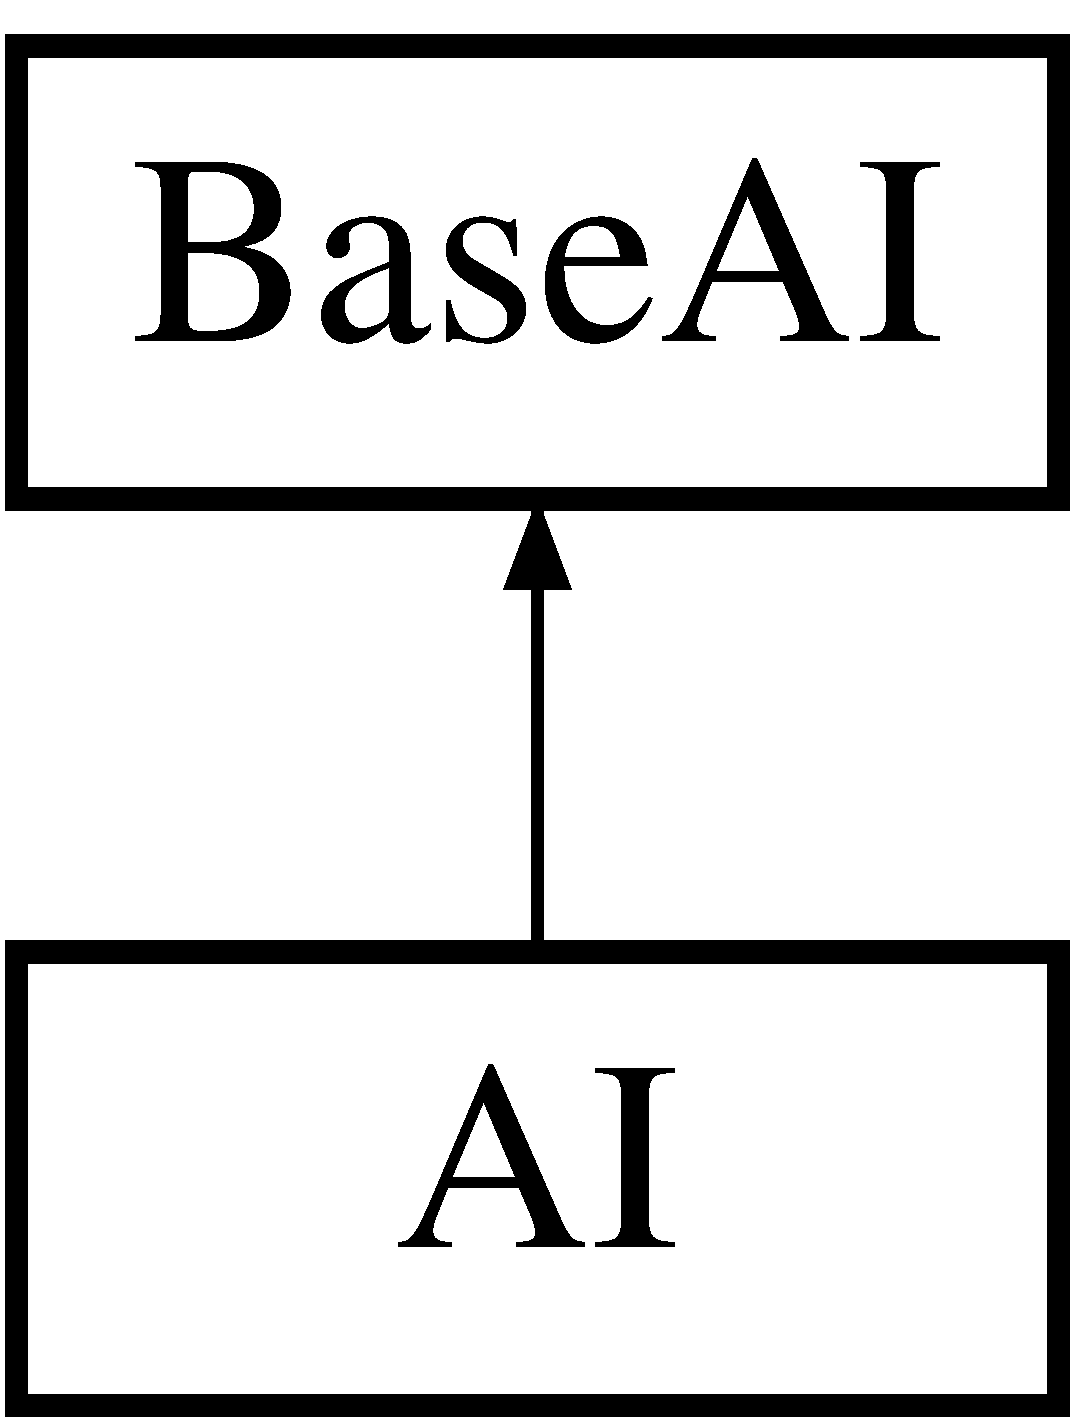
\includegraphics[height=2cm]{classAI}
\end{center}
\end{figure}
\subsection*{Public Member Functions}
\begin{DoxyCompactItemize}
\item 
\hypertarget{classAI_ae37d6a193873f7e35deb19671bf45a14}{
{\bfseries AI} (\hyperlink{structConnection}{Connection} $\ast$c)}
\label{classAI_ae37d6a193873f7e35deb19671bf45a14}

\item 
virtual const char $\ast$ \hyperlink{classAI_a529ac74a6f88a82abb1edd87847203e1}{username} ()
\item 
virtual const char $\ast$ \hyperlink{classAI_aa4e58e11bbbdb040e6b12f8706763a00}{password} ()
\item 
virtual void \hyperlink{classAI_a8c8e3a635791abaa61585357e6a25f63}{init} ()
\item 
virtual bool \hyperlink{classAI_a3c4746756b699cee5225597506521a39}{run} ()
\item 
virtual void \hyperlink{classAI_a67b00a8dd5c6d73db2e4e2332826462e}{end} ()
\item 
\hypertarget{classAI_ac4f1565ad6e33d6999663baf20c11861}{
void {\bfseries unload} (\hyperlink{classBot}{Bot} \&actor, \hyperlink{classUnit}{Unit} \&target)}
\label{classAI_ac4f1565ad6e33d6999663baf20c11861}

\item 
\hypertarget{classAI_a50bee5fc94b1d2b12fe2d960f3ed074b}{
bool {\bfseries inRange} (\hyperlink{classBot}{Bot} \&actor, \hyperlink{classUnit}{Unit} \&target)}
\label{classAI_a50bee5fc94b1d2b12fe2d960f3ed074b}

\item 
\hypertarget{classAI_ac8cee3de4faa8cb0b446a8494752f4ac}{
\hyperlink{classUnit}{Unit} $\ast$ {\bfseries findNearestTarget} (\hyperlink{classBot}{Bot} \&actor)}
\label{classAI_ac8cee3de4faa8cb0b446a8494752f4ac}

\item 
\hypertarget{classAI_a0162d0d17ab9dc076785b14de0bc8c37}{
void {\bfseries moveTowardsTarget} (\hyperlink{classBot}{Bot} \&actor, \hyperlink{classUnit}{Unit} \&target)}
\label{classAI_a0162d0d17ab9dc076785b14de0bc8c37}

\end{DoxyCompactItemize}


\subsection{Detailed Description}
The class implementing gameplay logic. 

\subsection{Member Function Documentation}
\hypertarget{classAI_a67b00a8dd5c6d73db2e4e2332826462e}{
\index{AI@{AI}!end@{end}}
\index{end@{end}!AI@{AI}}
\subsubsection[{end}]{\setlength{\rightskip}{0pt plus 5cm}void AI::end ()\hspace{0.3cm}{\ttfamily  \mbox{[}virtual\mbox{]}}}}
\label{classAI_a67b00a8dd5c6d73db2e4e2332826462e}
This function is called after the last turn. 

Implements \hyperlink{classBaseAI_a60c8246a859ba2dba84b70239bc129bc}{BaseAI}.

\hypertarget{classAI_a8c8e3a635791abaa61585357e6a25f63}{
\index{AI@{AI}!init@{init}}
\index{init@{init}!AI@{AI}}
\subsubsection[{init}]{\setlength{\rightskip}{0pt plus 5cm}void AI::init ()\hspace{0.3cm}{\ttfamily  \mbox{[}virtual\mbox{]}}}}
\label{classAI_a8c8e3a635791abaa61585357e6a25f63}
This function is run once, before your first turn. 

Implements \hyperlink{classBaseAI_a90ce8becd6f2e32c2cc32d41145e88df}{BaseAI}.

\hypertarget{classAI_aa4e58e11bbbdb040e6b12f8706763a00}{
\index{AI@{AI}!password@{password}}
\index{password@{password}!AI@{AI}}
\subsubsection[{password}]{\setlength{\rightskip}{0pt plus 5cm}const char $\ast$ AI::password ()\hspace{0.3cm}{\ttfamily  \mbox{[}virtual\mbox{]}}}}
\label{classAI_aa4e58e11bbbdb040e6b12f8706763a00}
Make this your password, which should be provided. 

Implements \hyperlink{classBaseAI_a9251e20447917cda64ad1487b903456f}{BaseAI}.

\hypertarget{classAI_a3c4746756b699cee5225597506521a39}{
\index{AI@{AI}!run@{run}}
\index{run@{run}!AI@{AI}}
\subsubsection[{run}]{\setlength{\rightskip}{0pt plus 5cm}bool AI::run ()\hspace{0.3cm}{\ttfamily  \mbox{[}virtual\mbox{]}}}}
\label{classAI_a3c4746756b699cee5225597506521a39}
This function is called each time it is your turn Return true to end your turn, return false to ask the server for updated information 

Implements \hyperlink{classBaseAI_ad60148e7e9e450ce47432b07b4db1ed6}{BaseAI}.

\hypertarget{classAI_a529ac74a6f88a82abb1edd87847203e1}{
\index{AI@{AI}!username@{username}}
\index{username@{username}!AI@{AI}}
\subsubsection[{username}]{\setlength{\rightskip}{0pt plus 5cm}const char $\ast$ AI::username ()\hspace{0.3cm}{\ttfamily  \mbox{[}virtual\mbox{]}}}}
\label{classAI_a529ac74a6f88a82abb1edd87847203e1}
Make this your username, which should be provided. 

Implements \hyperlink{classBaseAI_aef082fbf306fec04515ed5ed3b1ba582}{BaseAI}.



The documentation for this class was generated from the following files:\begin{DoxyCompactItemize}
\item 
AI.h\item 
AI.cpp\end{DoxyCompactItemize}

\hypertarget{classBaseAI}{
\section{BaseAI Class Reference}
\label{classBaseAI}\index{BaseAI@{BaseAI}}
}


A basic \hyperlink{classAI}{AI} interface.  


Inheritance diagram for BaseAI:\begin{figure}[H]
\begin{center}
\leavevmode
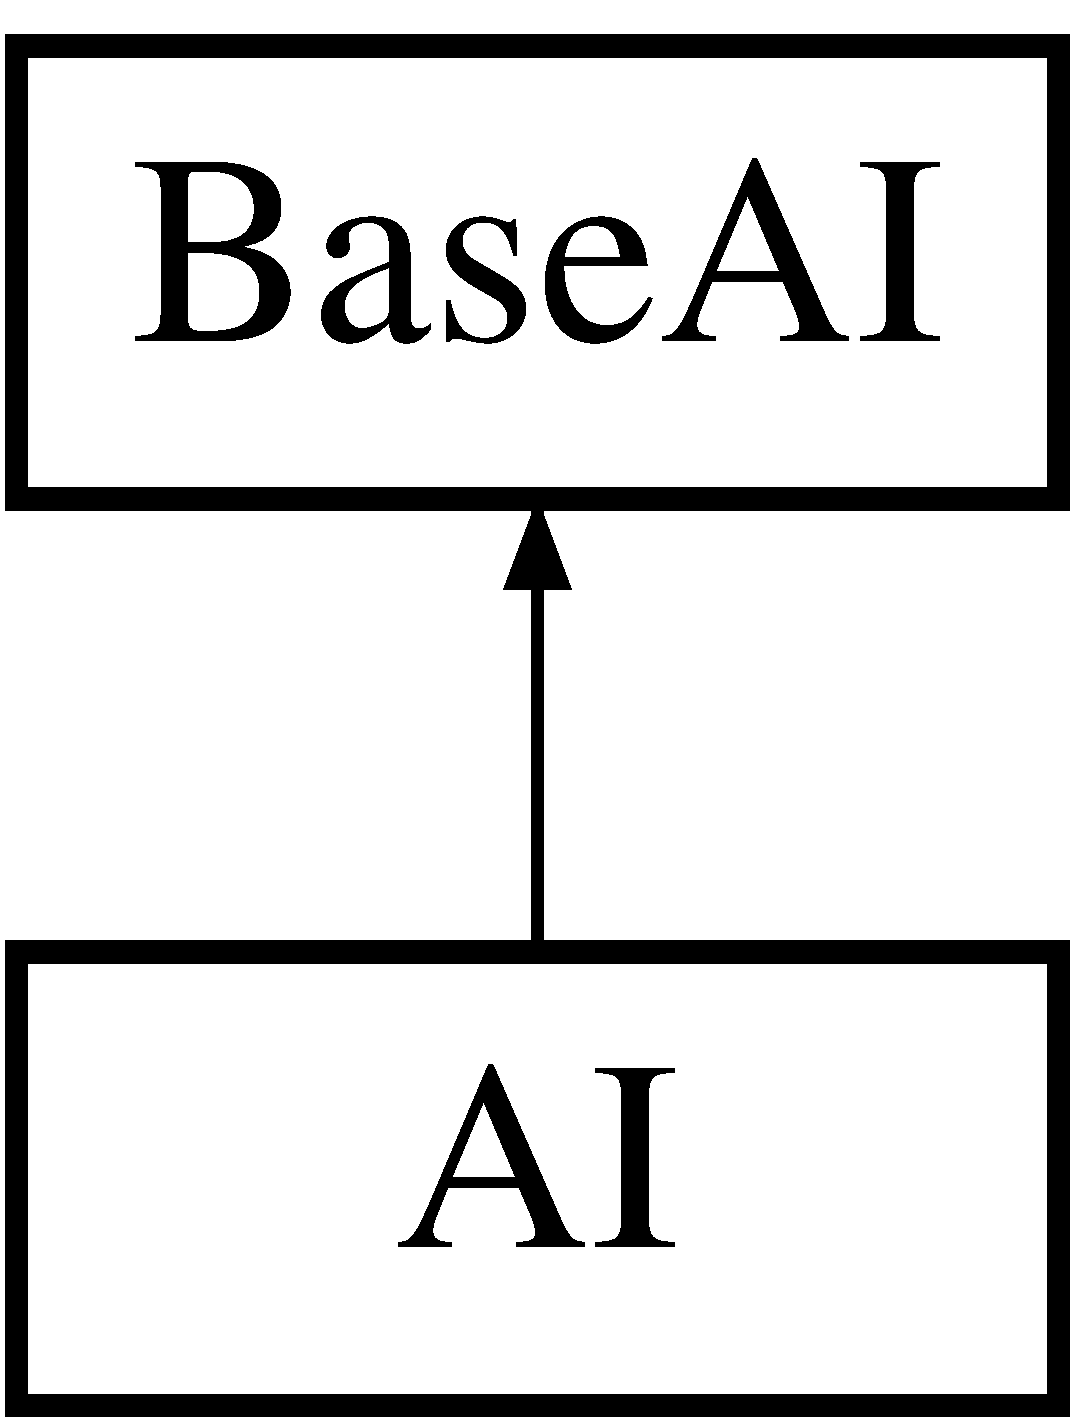
\includegraphics[height=2cm]{classBaseAI}
\end{center}
\end{figure}
\subsection*{Public Member Functions}
\begin{DoxyCompactItemize}
\item 
\hypertarget{classBaseAI_a27e93801ded2a4e1846f2b58beb37972}{
{\bfseries BaseAI} (Pointer c)}
\label{classBaseAI_a27e93801ded2a4e1846f2b58beb37972}

\item 
abstract String \hyperlink{classBaseAI_aa26770dd7db8dd0c4466dd770d4e05ba}{username} ()
\item 
abstract String \hyperlink{classBaseAI_a8607533e2b5bd9920ded593ae6509f48}{password} ()
\item 
abstract void \hyperlink{classBaseAI_a71b49f4ca248bfd32a9f9557cb6d494a}{init} ()
\item 
abstract boolean \hyperlink{classBaseAI_a56c96a58c1f1e93d17f9817711a45594}{run} ()
\item 
abstract void \hyperlink{classBaseAI_afb1c3a00ed081e9efdfff9f7d1e6910d}{end} ()
\item 
\hypertarget{classBaseAI_a862e05b3099817fcceb55beeef7225fe}{
boolean {\bfseries startTurn} ()}
\label{classBaseAI_a862e05b3099817fcceb55beeef7225fe}

\end{DoxyCompactItemize}
\subsection*{Package Functions}
\begin{DoxyCompactItemize}
\item 
\hypertarget{classBaseAI_a19ade7391bfe101884a35f48fb840199}{
int \hyperlink{classBaseAI_a19ade7391bfe101884a35f48fb840199}{turnNumber} ()}
\label{classBaseAI_a19ade7391bfe101884a35f48fb840199}

\begin{DoxyCompactList}\small\item\em How many turns it has been since the beginning of the game. \item\end{DoxyCompactList}\item 
\hypertarget{classBaseAI_a16aab1036653c8f8fb5370cf2f6a3e10}{
int \hyperlink{classBaseAI_a16aab1036653c8f8fb5370cf2f6a3e10}{playerID} ()}
\label{classBaseAI_a16aab1036653c8f8fb5370cf2f6a3e10}

\begin{DoxyCompactList}\small\item\em Player Number; either 0 or 1. \item\end{DoxyCompactList}\item 
\hypertarget{classBaseAI_a298c9ca7f754329796f45e38383c2c0a}{
int \hyperlink{classBaseAI_a298c9ca7f754329796f45e38383c2c0a}{boardX} ()}
\label{classBaseAI_a298c9ca7f754329796f45e38383c2c0a}

\begin{DoxyCompactList}\small\item\em Maximum valid position in the X (right) direction. (0,0) is top left. \item\end{DoxyCompactList}\item 
\hypertarget{classBaseAI_aaf123aaebe77eeda93c3d78d5783f541}{
int \hyperlink{classBaseAI_aaf123aaebe77eeda93c3d78d5783f541}{boardY} ()}
\label{classBaseAI_aaf123aaebe77eeda93c3d78d5783f541}

\begin{DoxyCompactList}\small\item\em Maximum valid position in the Y (down) direction. (0,0) is top left. \item\end{DoxyCompactList}\item 
\hypertarget{classBaseAI_a50d3091db33b93c6f7c2d11dd64b4c7a}{
int \hyperlink{classBaseAI_a50d3091db33b93c6f7c2d11dd64b4c7a}{gameNumber} ()}
\label{classBaseAI_a50d3091db33b93c6f7c2d11dd64b4c7a}

\begin{DoxyCompactList}\small\item\em What number game this is for the server. \item\end{DoxyCompactList}\item 
\hypertarget{classBaseAI_a0c98c065f57b1519d6daf72ef1c71d71}{
int \hyperlink{classBaseAI_a0c98c065f57b1519d6daf72ef1c71d71}{player0Time} ()}
\label{classBaseAI_a0c98c065f57b1519d6daf72ef1c71d71}

\begin{DoxyCompactList}\small\item\em Player 0's time remaining. \item\end{DoxyCompactList}\item 
\hypertarget{classBaseAI_a5a96b2451bf0e2f6567e9e56d59cf7cb}{
int \hyperlink{classBaseAI_a5a96b2451bf0e2f6567e9e56d59cf7cb}{player1Time} ()}
\label{classBaseAI_a5a96b2451bf0e2f6567e9e56d59cf7cb}

\begin{DoxyCompactList}\small\item\em Player 1's time remaining. \item\end{DoxyCompactList}\end{DoxyCompactItemize}
\subsection*{Package Attributes}
\begin{DoxyCompactItemize}
\item 
\hypertarget{classBaseAI_ad9836b270a011daee8411f84590ba35a}{
Pointer {\bfseries connection}}
\label{classBaseAI_ad9836b270a011daee8411f84590ba35a}

\item 
\hypertarget{classBaseAI_a94966bbfdac0d091a7332f19b29935c3}{
boolean {\bfseries initialized}}
\label{classBaseAI_a94966bbfdac0d091a7332f19b29935c3}

\end{DoxyCompactItemize}
\subsection*{Static Package Attributes}
\begin{DoxyCompactItemize}
\item 
\hypertarget{classBaseAI_a201fc0bad05f5cd5a8fa0c38d1b8f393}{
static \hyperlink{classBot}{Bot}\mbox{[}$\,$\mbox{]} {\bfseries bots}}
\label{classBaseAI_a201fc0bad05f5cd5a8fa0c38d1b8f393}

\item 
\hypertarget{classBaseAI_a858e9e6dead0b8b9dc2a13db34d66d5e}{
static \hyperlink{classFrame}{Frame}\mbox{[}$\,$\mbox{]} {\bfseries frames}}
\label{classBaseAI_a858e9e6dead0b8b9dc2a13db34d66d5e}

\item 
\hypertarget{classBaseAI_a5149adb4efc5b8fc7370b747592e2ae5}{
static \hyperlink{classWall}{Wall}\mbox{[}$\,$\mbox{]} {\bfseries walls}}
\label{classBaseAI_a5149adb4efc5b8fc7370b747592e2ae5}

\item 
\hypertarget{classBaseAI_a82450c46af1b8f5ef7b6470803105e5a}{
static \hyperlink{classType}{Type}\mbox{[}$\,$\mbox{]} {\bfseries types}}
\label{classBaseAI_a82450c46af1b8f5ef7b6470803105e5a}

\item 
\hypertarget{classBaseAI_ad7942cee117a347f7cb841ff4800408f}{
static int {\bfseries iteration}}
\label{classBaseAI_ad7942cee117a347f7cb841ff4800408f}

\end{DoxyCompactItemize}


\subsection{Detailed Description}
A basic \hyperlink{classAI}{AI} interface. This class implements most the code an \hyperlink{classAI}{AI} would need to interface with the lower-\/level game code. AIs should extend this class to get a lot of builer-\/plate code out of the way The provided \hyperlink{classAI}{AI} class does just that. 

\subsection{Member Function Documentation}
\hypertarget{classBaseAI_afb1c3a00ed081e9efdfff9f7d1e6910d}{
\index{BaseAI@{BaseAI}!end@{end}}
\index{end@{end}!BaseAI@{BaseAI}}
\subsubsection[{end}]{\setlength{\rightskip}{0pt plus 5cm}abstract void BaseAI::end ()\hspace{0.3cm}{\ttfamily  \mbox{[}pure virtual\mbox{]}}}}
\label{classBaseAI_afb1c3a00ed081e9efdfff9f7d1e6910d}
This is run on after your last turn. 

Implemented in \hyperlink{classAI_a67b00a8dd5c6d73db2e4e2332826462e}{AI}.

\hypertarget{classBaseAI_a71b49f4ca248bfd32a9f9557cb6d494a}{
\index{BaseAI@{BaseAI}!init@{init}}
\index{init@{init}!BaseAI@{BaseAI}}
\subsubsection[{init}]{\setlength{\rightskip}{0pt plus 5cm}abstract void BaseAI::init ()\hspace{0.3cm}{\ttfamily  \mbox{[}pure virtual\mbox{]}}}}
\label{classBaseAI_a71b49f4ca248bfd32a9f9557cb6d494a}
This is run on turn 1 before run 

Implemented in \hyperlink{classAI_a8c8e3a635791abaa61585357e6a25f63}{AI}.

\hypertarget{classBaseAI_a8607533e2b5bd9920ded593ae6509f48}{
\index{BaseAI@{BaseAI}!password@{password}}
\index{password@{password}!BaseAI@{BaseAI}}
\subsubsection[{password}]{\setlength{\rightskip}{0pt plus 5cm}abstract String BaseAI::password ()\hspace{0.3cm}{\ttfamily  \mbox{[}pure virtual\mbox{]}}}}
\label{classBaseAI_a8607533e2b5bd9920ded593ae6509f48}
Make this your password, which should be provided. 

Implemented in \hyperlink{classAI_a405047fd39e03de993183392a06d655b}{AI}.

\hypertarget{classBaseAI_a56c96a58c1f1e93d17f9817711a45594}{
\index{BaseAI@{BaseAI}!run@{run}}
\index{run@{run}!BaseAI@{BaseAI}}
\subsubsection[{run}]{\setlength{\rightskip}{0pt plus 5cm}abstract boolean BaseAI::run ()\hspace{0.3cm}{\ttfamily  \mbox{[}pure virtual\mbox{]}}}}
\label{classBaseAI_a56c96a58c1f1e93d17f9817711a45594}
This is run every turn . Return true to end the turn, return false to request a status update from the server and then immediately rerun this function with the latest game status. 

Implemented in \hyperlink{classAI_af25b3a076daef2aaf9f74ecf458bdfbc}{AI}.

\hypertarget{classBaseAI_aa26770dd7db8dd0c4466dd770d4e05ba}{
\index{BaseAI@{BaseAI}!username@{username}}
\index{username@{username}!BaseAI@{BaseAI}}
\subsubsection[{username}]{\setlength{\rightskip}{0pt plus 5cm}abstract String BaseAI::username ()\hspace{0.3cm}{\ttfamily  \mbox{[}pure virtual\mbox{]}}}}
\label{classBaseAI_aa26770dd7db8dd0c4466dd770d4e05ba}
Make this your username, which should be provided. 

Implemented in \hyperlink{classAI_ad7e6db6b414a192ad2af8656d012cfdc}{AI}.



The documentation for this class was generated from the following file:\begin{DoxyCompactItemize}
\item 
BaseAI.java\end{DoxyCompactItemize}

\hypertarget{classBot}{
\section{Bot Class Reference}
\label{classBot}\index{Bot@{Bot}}
}


The bot class.  




{\ttfamily \#include $<$Bot.h$>$}

Inheritance diagram for Bot:\begin{figure}[H]
\begin{center}
\leavevmode
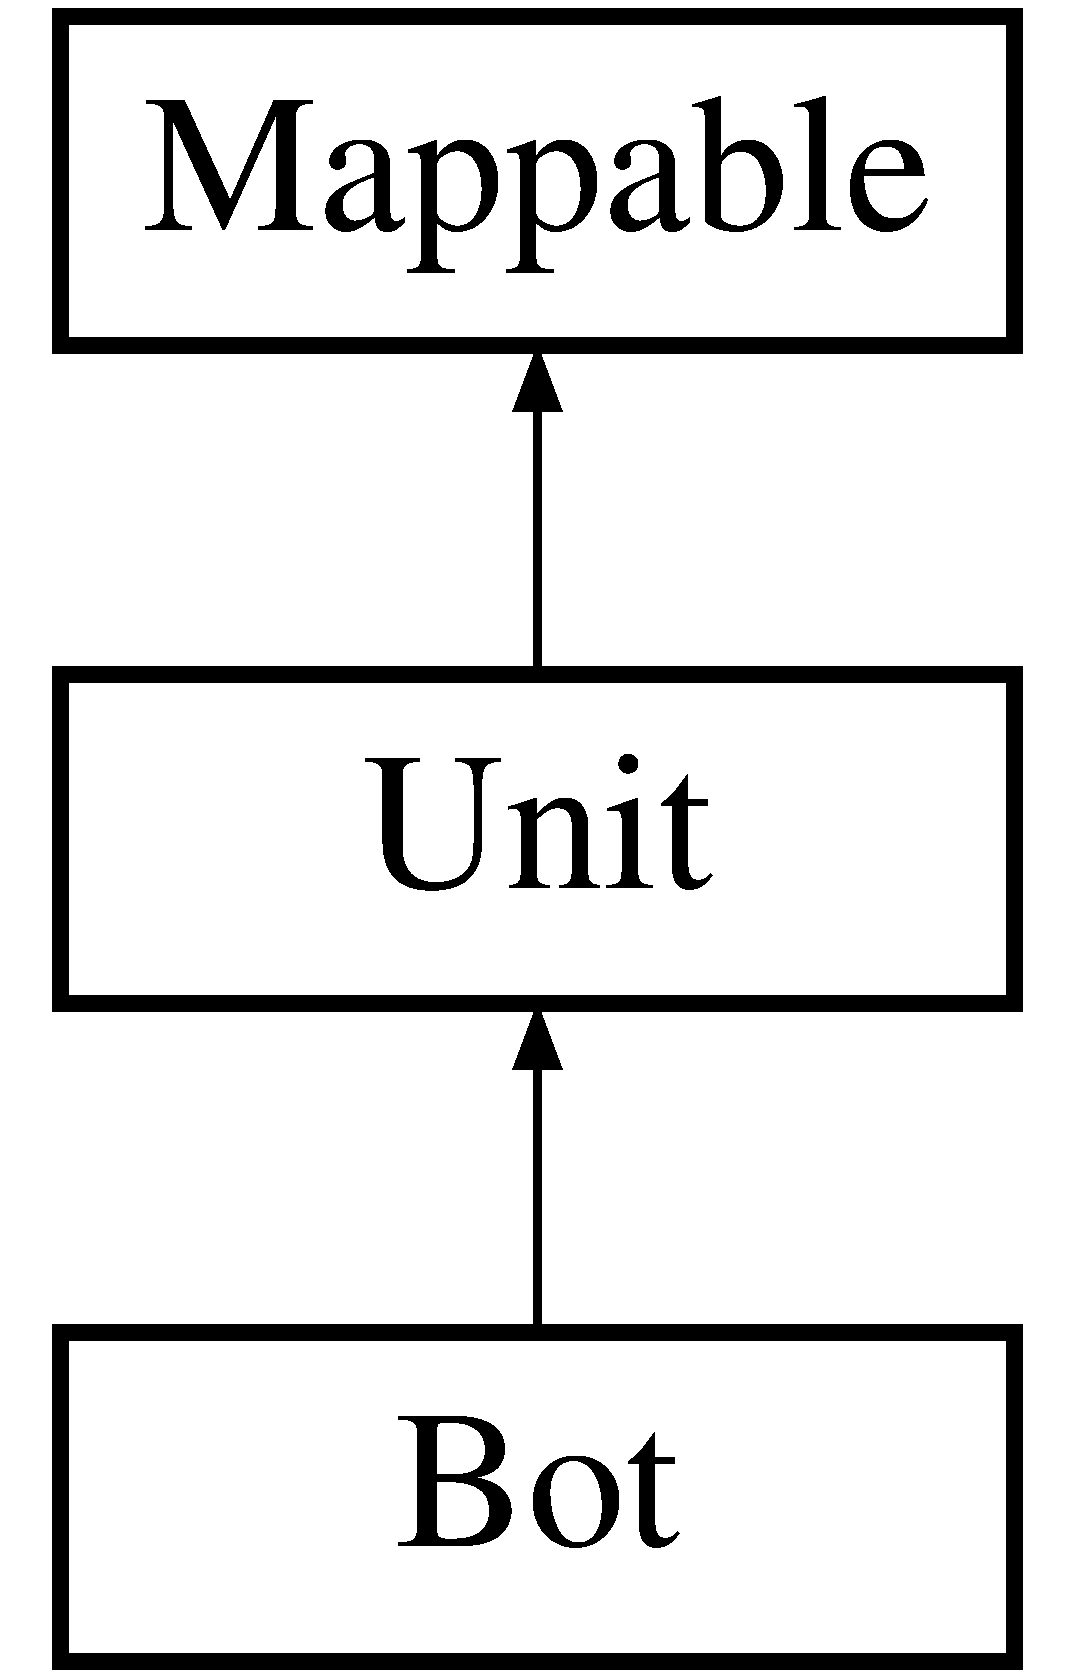
\includegraphics[height=3cm]{classBot}
\end{center}
\end{figure}
\subsection*{Public Member Functions}
\begin{DoxyCompactItemize}
\item 
\hypertarget{classBot_a5b75fd7e8eb162952a00394a3baff2df}{
{\bfseries Bot} (\hyperlink{struct__Bot}{\_\-Bot} $\ast$ptr=NULL)}
\label{classBot_a5b75fd7e8eb162952a00394a3baff2df}

\item 
\hypertarget{classBot_a465fcc505b25a8bd189abae0a08f903e}{
int \hyperlink{classBot_a465fcc505b25a8bd189abae0a08f903e}{id} ()}
\label{classBot_a465fcc505b25a8bd189abae0a08f903e}

\begin{DoxyCompactList}\small\item\em Unique Identifier. \item\end{DoxyCompactList}\item 
\hypertarget{classBot_aa2a50ed336378c5bf065fd69a42f147c}{
int \hyperlink{classBot_aa2a50ed336378c5bf065fd69a42f147c}{x} ()}
\label{classBot_aa2a50ed336378c5bf065fd69a42f147c}

\begin{DoxyCompactList}\small\item\em The X position of the top left corner of this object. X is horizontal. \item\end{DoxyCompactList}\item 
\hypertarget{classBot_a5d5c81be976e3dec23a378032fc290a2}{
int \hyperlink{classBot_a5d5c81be976e3dec23a378032fc290a2}{y} ()}
\label{classBot_a5d5c81be976e3dec23a378032fc290a2}

\begin{DoxyCompactList}\small\item\em The Y position of the top left corner of this object. Y is vertical. \item\end{DoxyCompactList}\item 
\hypertarget{classBot_ae8d6798379f4552dcc619c3a4b9744aa}{
int \hyperlink{classBot_ae8d6798379f4552dcc619c3a4b9744aa}{owner} ()}
\label{classBot_ae8d6798379f4552dcc619c3a4b9744aa}

\begin{DoxyCompactList}\small\item\em The owning player. \item\end{DoxyCompactList}\item 
\hypertarget{classBot_a0eecab2259afa7b3aeb596cccfcc4915}{
int \hyperlink{classBot_a0eecab2259afa7b3aeb596cccfcc4915}{health} ()}
\label{classBot_a0eecab2259afa7b3aeb596cccfcc4915}

\begin{DoxyCompactList}\small\item\em How much health this unit currently has. \item\end{DoxyCompactList}\item 
\hypertarget{classBot_a5da61adb4275e225cf2293a91701cac2}{
int \hyperlink{classBot_a5da61adb4275e225cf2293a91701cac2}{maxHealth} ()}
\label{classBot_a5da61adb4275e225cf2293a91701cac2}

\begin{DoxyCompactList}\small\item\em The maximum amount of health this unit can ever have. \item\end{DoxyCompactList}\item 
\hypertarget{classBot_ac11195160a92b68eb5cce1a5c100395b}{
int \hyperlink{classBot_ac11195160a92b68eb5cce1a5c100395b}{actions} ()}
\label{classBot_ac11195160a92b68eb5cce1a5c100395b}

\begin{DoxyCompactList}\small\item\em How many actions this bot can still perform. \item\end{DoxyCompactList}\item 
\hypertarget{classBot_a9ac3ebfa1429eb945ac0a00ea642ba41}{
int \hyperlink{classBot_a9ac3ebfa1429eb945ac0a00ea642ba41}{steps} ()}
\label{classBot_a9ac3ebfa1429eb945ac0a00ea642ba41}

\begin{DoxyCompactList}\small\item\em How many steps this bot can still take. \item\end{DoxyCompactList}\item 
\hypertarget{classBot_a7231a6a603986259558366bfb59ada0a}{
int \hyperlink{classBot_a7231a6a603986259558366bfb59ada0a}{size} ()}
\label{classBot_a7231a6a603986259558366bfb59ada0a}

\begin{DoxyCompactList}\small\item\em The length of one side of this robot, such that size$^\wedge$2 = number of bots combined into this bot. \item\end{DoxyCompactList}\item 
\hypertarget{classBot_a565185d07dfbc75377c1f97eadb6a871}{
int \hyperlink{classBot_a565185d07dfbc75377c1f97eadb6a871}{damage} ()}
\label{classBot_a565185d07dfbc75377c1f97eadb6a871}

\begin{DoxyCompactList}\small\item\em The amount of damage this robot does when attacking. \item\end{DoxyCompactList}\item 
\hypertarget{classBot_a8fd584436d258d25f09cc535f53a6775}{
int \hyperlink{classBot_a8fd584436d258d25f09cc535f53a6775}{range} ()}
\label{classBot_a8fd584436d258d25f09cc535f53a6775}

\begin{DoxyCompactList}\small\item\em How far this robot can attack or heal from its edge. \item\end{DoxyCompactList}\item 
\hypertarget{classBot_a49a96305ac775de2b31ceef370ae135a}{
int \hyperlink{classBot_a49a96305ac775de2b31ceef370ae135a}{movitude} ()}
\label{classBot_a49a96305ac775de2b31ceef370ae135a}

\begin{DoxyCompactList}\small\item\em This value divided by the number of bots = maxSteps for this robot. \item\end{DoxyCompactList}\item 
\hypertarget{classBot_a87733c9b7400d2df33f07d38dad54a41}{
int \hyperlink{classBot_a87733c9b7400d2df33f07d38dad54a41}{actitude} ()}
\label{classBot_a87733c9b7400d2df33f07d38dad54a41}

\begin{DoxyCompactList}\small\item\em This value divided by the number of bots = maxActions for this robot. \item\end{DoxyCompactList}\item 
\hypertarget{classBot_aa30cc3cea31e7322bcc38c2cba1472d6}{
int \hyperlink{classBot_aa30cc3cea31e7322bcc38c2cba1472d6}{buildRate} ()}
\label{classBot_aa30cc3cea31e7322bcc38c2cba1472d6}

\begin{DoxyCompactList}\small\item\em This value is used to determine how many turns it takes to build a robot and how much this robot heals for. \item\end{DoxyCompactList}\item 
\hypertarget{classBot_a7cd6d04cbcfb705202350cfc7310c9af}{
int \hyperlink{classBot_a7cd6d04cbcfb705202350cfc7310c9af}{partOf} ()}
\label{classBot_a7cd6d04cbcfb705202350cfc7310c9af}

\begin{DoxyCompactList}\small\item\em ID of the robot this robot is apart of, 0 if not in a robot. \item\end{DoxyCompactList}\item 
\hypertarget{classBot_a20891617ea241884bf1cd3642914a660}{
int \hyperlink{classBot_a20891617ea241884bf1cd3642914a660}{building} ()}
\label{classBot_a20891617ea241884bf1cd3642914a660}

\begin{DoxyCompactList}\small\item\em ID of the robot this robot is building, 0 if not building. \item\end{DoxyCompactList}\item 
\hypertarget{classBot_a85dc8bb8e995c5c40468225ccaa5ebbd}{
int \hyperlink{classBot_a85dc8bb8e995c5c40468225ccaa5ebbd}{type} ()}
\label{classBot_a85dc8bb8e995c5c40468225ccaa5ebbd}

\begin{DoxyCompactList}\small\item\em ID of the type this robot is, 0 if a combination. \item\end{DoxyCompactList}\item 
\hypertarget{classBot_a168f5c58ade8b9fc6dc88340b046e314}{
int \hyperlink{classBot_a168f5c58ade8b9fc6dc88340b046e314}{talk} (std::string message)}
\label{classBot_a168f5c58ade8b9fc6dc88340b046e314}

\begin{DoxyCompactList}\small\item\em Sends a message to be visualized when this unit is selected. \item\end{DoxyCompactList}\item 
\hypertarget{classBot_a15d55cdd01ddcf65b0f84a9e74f35ffa}{
int \hyperlink{classBot_a15d55cdd01ddcf65b0f84a9e74f35ffa}{move} (std::string direction)}
\label{classBot_a15d55cdd01ddcf65b0f84a9e74f35ffa}

\begin{DoxyCompactList}\small\item\em Move in the indicated direction (U, D, L, or R). U is y=y-\/1, L=x=x-\/1, such that the top left corner is (0,0). Requires the calling robot to have a step. \item\end{DoxyCompactList}\item 
\hypertarget{classBot_af877960466913d96dc12b7363b70fb38}{
int \hyperlink{classBot_af877960466913d96dc12b7363b70fb38}{attack} (\hyperlink{classUnit}{Unit} \&target)}
\label{classBot_af877960466913d96dc12b7363b70fb38}

\begin{DoxyCompactList}\small\item\em Attack the specified unit. Requires the calling robot to have an action and for the target to be in range. \item\end{DoxyCompactList}\item 
\hypertarget{classBot_afac1a68fc38adf0384730d08e6e73c45}{
int \hyperlink{classBot_afac1a68fc38adf0384730d08e6e73c45}{heal} (\hyperlink{classBot}{Bot} \&target)}
\label{classBot_afac1a68fc38adf0384730d08e6e73c45}

\begin{DoxyCompactList}\small\item\em Heals the indicated bot. Requires the calling robot to have an action and for the target to be in range. Heals for target.maxHealth $\ast$ self.buildRate / (4 $\ast$ target.size$^\wedge$2). \item\end{DoxyCompactList}\item 
\hypertarget{classBot_a705ebce4a19f93bf6d8edc02fb70f1f7}{
int \hyperlink{classBot_a705ebce4a19f93bf6d8edc02fb70f1f7}{build} (\hyperlink{classType}{Type} \&type, int x, int y, int size)}
\label{classBot_a705ebce4a19f93bf6d8edc02fb70f1f7}

\begin{DoxyCompactList}\small\item\em Begins building a new robot. While building, the new robot will be a frame. Requires the calling robot to have an action. X and Y must cause the new robot to be adjacent. Size must be less than or equal to the calling robots size. Completes in 8 $\ast$ size$^\wedge$2 / self.buildRate turns. \item\end{DoxyCompactList}\item 
\hypertarget{classBot_a9e0de3afc7548e660818e937125fb76d}{
int \hyperlink{classBot_a9e0de3afc7548e660818e937125fb76d}{combine} (\hyperlink{classBot}{Bot} \&bot2, \hyperlink{classBot}{Bot} \&bot3, \hyperlink{classBot}{Bot} \&bot4)}
\label{classBot_a9e0de3afc7548e660818e937125fb76d}

\begin{DoxyCompactList}\small\item\em Combines four robots into one. Requires all robots to have an action, be of the same size, and be arranged in a square. \item\end{DoxyCompactList}\item 
\hypertarget{classBot_ad710db985160136aa8e3c624b26afc4e}{
int \hyperlink{classBot_ad710db985160136aa8e3c624b26afc4e}{split} ()}
\label{classBot_ad710db985160136aa8e3c624b26afc4e}

\begin{DoxyCompactList}\small\item\em Splits a compound bot into the 4 robots that combined to make it. Requires the calling robot to have an action. \item\end{DoxyCompactList}\item 
\hypertarget{classBot_a49f602d6258372ec647d53aa3fc6f85f}{
int \hyperlink{classBot_a49f602d6258372ec647d53aa3fc6f85f}{maxActions} ()}
\label{classBot_a49f602d6258372ec647d53aa3fc6f85f}

\begin{DoxyCompactList}\small\item\em Returns the maximum number of actions this robot can take per turn. \item\end{DoxyCompactList}\item 
\hypertarget{classBot_a620c2dc2c13fc027e1611c2d84b655b7}{
int \hyperlink{classBot_a620c2dc2c13fc027e1611c2d84b655b7}{maxSteps} ()}
\label{classBot_a620c2dc2c13fc027e1611c2d84b655b7}

\begin{DoxyCompactList}\small\item\em Returns the maximum number of steps this robot can take per turn. \item\end{DoxyCompactList}\end{DoxyCompactItemize}
\subsection*{Friends}
\begin{DoxyCompactItemize}
\item 
\hypertarget{classBot_a3651bfa118ec5110648a3804b2dfaca4}{
std::ostream \& {\bfseries operator$<$$<$} (std::ostream \&stream, \hyperlink{classBot}{Bot} ob)}
\label{classBot_a3651bfa118ec5110648a3804b2dfaca4}

\end{DoxyCompactItemize}


\subsection{Detailed Description}
The bot class. 

The documentation for this class was generated from the following files:\begin{DoxyCompactItemize}
\item 
Bot.h\item 
Bot.cpp\end{DoxyCompactItemize}

\hypertarget{structConnection}{
\section{Connection Struct Reference}
\label{structConnection}\index{Connection@{Connection}}
}
\subsection*{Public Attributes}
\begin{DoxyCompactItemize}
\item 
\hypertarget{structConnection_afeebe9a1ebc19966d58faa5eca7ad36d}{
int {\bfseries socket}}
\label{structConnection_afeebe9a1ebc19966d58faa5eca7ad36d}

\item 
\hypertarget{structConnection_a7b27ff790f8a42a54c76ef4d163d7e57}{
pthread\_\-mutex\_\-t {\bfseries mutex}}
\label{structConnection_a7b27ff790f8a42a54c76ef4d163d7e57}

\item 
\hypertarget{structConnection_ae1f13fe61a2400a6a1cc9322f25d286b}{
int {\bfseries turnNumber}}
\label{structConnection_ae1f13fe61a2400a6a1cc9322f25d286b}

\item 
\hypertarget{structConnection_a8054101484b1635e9e2888390fc7e82d}{
int {\bfseries playerID}}
\label{structConnection_a8054101484b1635e9e2888390fc7e82d}

\item 
\hypertarget{structConnection_a915028dcc52b6cd72678fed892bf0834}{
int {\bfseries boardX}}
\label{structConnection_a915028dcc52b6cd72678fed892bf0834}

\item 
\hypertarget{structConnection_aca78001bac4a1d2433ee5f65ba1260d8}{
int {\bfseries boardY}}
\label{structConnection_aca78001bac4a1d2433ee5f65ba1260d8}

\item 
\hypertarget{structConnection_a33a204e9624fbd7b0a77347a15ec0f10}{
int {\bfseries gameNumber}}
\label{structConnection_a33a204e9624fbd7b0a77347a15ec0f10}

\item 
\hypertarget{structConnection_a214b3530af5b40ec1abd7b6817770a3e}{
int {\bfseries player0Time}}
\label{structConnection_a214b3530af5b40ec1abd7b6817770a3e}

\item 
\hypertarget{structConnection_a0adf2a815f73e16206d911f63caededa}{
int {\bfseries player1Time}}
\label{structConnection_a0adf2a815f73e16206d911f63caededa}

\item 
\hypertarget{structConnection_a6199df3cf201346b6e1d664791bad969}{
char $\ast$ {\bfseries player0Name}}
\label{structConnection_a6199df3cf201346b6e1d664791bad969}

\item 
\hypertarget{structConnection_aca48a06e1bff67f7e6796e3064ab29ef}{
char $\ast$ {\bfseries player1Name}}
\label{structConnection_aca48a06e1bff67f7e6796e3064ab29ef}

\item 
\hypertarget{structConnection_a72a03a6f80a270ad1e30a8cc00f82954}{
\hyperlink{struct__Bot}{\_\-Bot} $\ast$ {\bfseries Bots}}
\label{structConnection_a72a03a6f80a270ad1e30a8cc00f82954}

\item 
\hypertarget{structConnection_ab8b37a7a1b87d6c61a1736842d250342}{
int {\bfseries BotCount}}
\label{structConnection_ab8b37a7a1b87d6c61a1736842d250342}

\item 
\hypertarget{structConnection_ae65ec3fec853941f2138f0f2a0902d19}{
\hyperlink{struct__Frame}{\_\-Frame} $\ast$ {\bfseries Frames}}
\label{structConnection_ae65ec3fec853941f2138f0f2a0902d19}

\item 
\hypertarget{structConnection_a589e0384f35b61f26fee5d184810439e}{
int {\bfseries FrameCount}}
\label{structConnection_a589e0384f35b61f26fee5d184810439e}

\item 
\hypertarget{structConnection_a81490983ad40f32c911f16153d8133d7}{
\hyperlink{struct__Wall}{\_\-Wall} $\ast$ {\bfseries Walls}}
\label{structConnection_a81490983ad40f32c911f16153d8133d7}

\item 
\hypertarget{structConnection_a2a797a8b50d577633c99529b4faeb1a3}{
int {\bfseries WallCount}}
\label{structConnection_a2a797a8b50d577633c99529b4faeb1a3}

\item 
\hypertarget{structConnection_a6f2a2b2fc4e0e04d1154a2384d815609}{
\hyperlink{struct__Type}{\_\-Type} $\ast$ {\bfseries Types}}
\label{structConnection_a6f2a2b2fc4e0e04d1154a2384d815609}

\item 
\hypertarget{structConnection_a676cbda78a450c88795f1df5e6ce4d67}{
int {\bfseries TypeCount}}
\label{structConnection_a676cbda78a450c88795f1df5e6ce4d67}

\end{DoxyCompactItemize}


The documentation for this struct was generated from the following file:\begin{DoxyCompactItemize}
\item 
game.h\end{DoxyCompactItemize}

\hypertarget{classFrame}{
\section{Frame Class Reference}
\label{classFrame}\index{Frame@{Frame}}
}


A baby robot.  


\subsection*{Public Member Functions}
\begin{DoxyCompactItemize}
\item 
\hypertarget{classFrame_aec793ebd2605aebd01d46598f29267bd}{
{\bfseries Frame} (Pointer p)}
\label{classFrame_aec793ebd2605aebd01d46598f29267bd}

\item 
\hypertarget{classFrame_ade874be014eebf236ee2ff519d1e7f4c}{
int \hyperlink{classFrame_ade874be014eebf236ee2ff519d1e7f4c}{getId} ()}
\label{classFrame_ade874be014eebf236ee2ff519d1e7f4c}

\begin{DoxyCompactList}\small\item\em Unique Identifier. \item\end{DoxyCompactList}\item 
\hypertarget{classFrame_ac75792df8c0997a6251b67b5b19cdaf3}{
int \hyperlink{classFrame_ac75792df8c0997a6251b67b5b19cdaf3}{getX} ()}
\label{classFrame_ac75792df8c0997a6251b67b5b19cdaf3}

\begin{DoxyCompactList}\small\item\em The X position of the top left corner of this object. X is horizontal. \item\end{DoxyCompactList}\item 
\hypertarget{classFrame_a2cf0bdc9ac8f95db156493848be32915}{
int \hyperlink{classFrame_a2cf0bdc9ac8f95db156493848be32915}{getY} ()}
\label{classFrame_a2cf0bdc9ac8f95db156493848be32915}

\begin{DoxyCompactList}\small\item\em The Y position of the top left corner of this object. Y is vertical. \item\end{DoxyCompactList}\item 
\hypertarget{classFrame_a13edeeab79fa4a59353aabc5de650cd3}{
int \hyperlink{classFrame_a13edeeab79fa4a59353aabc5de650cd3}{getOwner} ()}
\label{classFrame_a13edeeab79fa4a59353aabc5de650cd3}

\begin{DoxyCompactList}\small\item\em The owning player. \item\end{DoxyCompactList}\item 
\hypertarget{classFrame_abc3cc9a10ea4a7255469c58577fc96f7}{
int \hyperlink{classFrame_abc3cc9a10ea4a7255469c58577fc96f7}{getHealth} ()}
\label{classFrame_abc3cc9a10ea4a7255469c58577fc96f7}

\begin{DoxyCompactList}\small\item\em How much health this unit currently has. \item\end{DoxyCompactList}\item 
\hypertarget{classFrame_ad0927f019898a2c9ac8c393bf689c405}{
int \hyperlink{classFrame_ad0927f019898a2c9ac8c393bf689c405}{getMaxHealth} ()}
\label{classFrame_ad0927f019898a2c9ac8c393bf689c405}

\begin{DoxyCompactList}\small\item\em The maximum amount of health this unit can ever have. \item\end{DoxyCompactList}\item 
\hypertarget{classFrame_a9718321b001d44f30579872c89040235}{
Pointer \hyperlink{classFrame_a9718321b001d44f30579872c89040235}{getType} ()}
\label{classFrame_a9718321b001d44f30579872c89040235}

\begin{DoxyCompactList}\small\item\em What type this robot will be. \item\end{DoxyCompactList}\item 
\hypertarget{classFrame_a4bf9dbcceb0540169c97c13b16a3ba83}{
int \hyperlink{classFrame_a4bf9dbcceb0540169c97c13b16a3ba83}{getSize} ()}
\label{classFrame_a4bf9dbcceb0540169c97c13b16a3ba83}

\begin{DoxyCompactList}\small\item\em The length of one side of this robot, such that size$^\wedge$2 = number of bots combined into this bot. \item\end{DoxyCompactList}\item 
\hypertarget{classFrame_ae3b0d040c3bc3e056cfca17195103078}{
int \hyperlink{classFrame_ae3b0d040c3bc3e056cfca17195103078}{getCompletionTime} ()}
\label{classFrame_ae3b0d040c3bc3e056cfca17195103078}

\begin{DoxyCompactList}\small\item\em How many of your turns until this frame becomes a robot. \item\end{DoxyCompactList}\end{DoxyCompactItemize}
\subsection*{Package Functions}
\begin{DoxyCompactItemize}
\item 
\hypertarget{classFrame_a1705d796a69b7ee777a6c7187ebdfbba}{
boolean {\bfseries validify} ()}
\label{classFrame_a1705d796a69b7ee777a6c7187ebdfbba}

\item 
\hypertarget{classFrame_a4932503ee86624433ff3475c9a3f0c5d}{
int \hyperlink{classFrame_a4932503ee86624433ff3475c9a3f0c5d}{talk} (String message)}
\label{classFrame_a4932503ee86624433ff3475c9a3f0c5d}

\begin{DoxyCompactList}\small\item\em Sends a message to be visualized when this unit is selected. \item\end{DoxyCompactList}\end{DoxyCompactItemize}
\subsection*{Package Attributes}
\begin{DoxyCompactItemize}
\item 
\hypertarget{classFrame_af3aed029f61190680a0cedbd2cbdde9c}{
Pointer {\bfseries ptr}}
\label{classFrame_af3aed029f61190680a0cedbd2cbdde9c}

\item 
\hypertarget{classFrame_a9a8d3de2300c27f2ab32341392c24416}{
int {\bfseries ID}}
\label{classFrame_a9a8d3de2300c27f2ab32341392c24416}

\item 
\hypertarget{classFrame_a9a5037560764dff9656616f337902ea8}{
int {\bfseries iteration}}
\label{classFrame_a9a5037560764dff9656616f337902ea8}

\end{DoxyCompactItemize}


\subsection{Detailed Description}
A baby robot. 

The documentation for this class was generated from the following file:\begin{DoxyCompactItemize}
\item 
Frame.java\end{DoxyCompactItemize}

\hypertarget{classMappable}{
\section{Mappable Class Reference}
\label{classMappable}\index{Mappable@{Mappable}}
}


An object that exists on the grid.  




{\ttfamily \#include $<$Mappable.h$>$}

Inheritance diagram for Mappable:\begin{figure}[H]
\begin{center}
\leavevmode
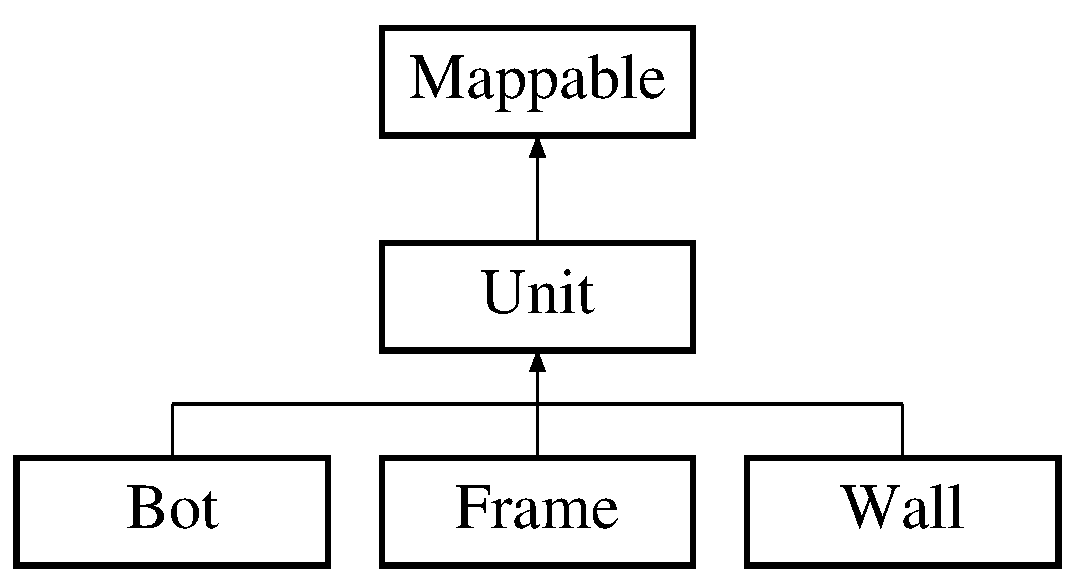
\includegraphics[height=3cm]{classMappable}
\end{center}
\end{figure}
\subsection*{Public Member Functions}
\begin{DoxyCompactItemize}
\item 
\hypertarget{classMappable_abb17854ba5e1c7d295c7277498227b80}{
{\bfseries Mappable} (\hyperlink{struct__Mappable}{\_\-Mappable} $\ast$ptr=NULL)}
\label{classMappable_abb17854ba5e1c7d295c7277498227b80}

\item 
\hypertarget{classMappable_a32bdecfde44acd6ac6eaecad2a2f7c25}{
int \hyperlink{classMappable_a32bdecfde44acd6ac6eaecad2a2f7c25}{id} ()}
\label{classMappable_a32bdecfde44acd6ac6eaecad2a2f7c25}

\begin{DoxyCompactList}\small\item\em Unique Identifier. \item\end{DoxyCompactList}\item 
\hypertarget{classMappable_a5295c64e0fb8536fac76f6722f28d051}{
int \hyperlink{classMappable_a5295c64e0fb8536fac76f6722f28d051}{x} ()}
\label{classMappable_a5295c64e0fb8536fac76f6722f28d051}

\begin{DoxyCompactList}\small\item\em The X position of the top left corner of this object. X is horizontal. \item\end{DoxyCompactList}\item 
\hypertarget{classMappable_a9beaf7680b58a574d8ee102a85c2cb9e}{
int \hyperlink{classMappable_a9beaf7680b58a574d8ee102a85c2cb9e}{y} ()}
\label{classMappable_a9beaf7680b58a574d8ee102a85c2cb9e}

\begin{DoxyCompactList}\small\item\em The Y position of the top left corner of this object. Y is vertical. \item\end{DoxyCompactList}\end{DoxyCompactItemize}
\subsection*{Public Attributes}
\begin{DoxyCompactItemize}
\item 
\hypertarget{classMappable_a8d9f478e553703116d7f636f19461de4}{
void $\ast$ {\bfseries ptr}}
\label{classMappable_a8d9f478e553703116d7f636f19461de4}

\end{DoxyCompactItemize}
\subsection*{Friends}
\begin{DoxyCompactItemize}
\item 
\hypertarget{classMappable_a0b57649bb1e7774386e133f026d60176}{
std::ostream \& {\bfseries operator$<$$<$} (std::ostream \&stream, \hyperlink{classMappable}{Mappable} ob)}
\label{classMappable_a0b57649bb1e7774386e133f026d60176}

\end{DoxyCompactItemize}


\subsection{Detailed Description}
An object that exists on the grid. 

The documentation for this class was generated from the following files:\begin{DoxyCompactItemize}
\item 
Mappable.h\item 
Mappable.cpp\end{DoxyCompactItemize}

\hypertarget{classType}{
\section{Type Class Reference}
\label{classType}\index{Type@{Type}}
}


A kind of robot.  


\subsection*{Public Member Functions}
\begin{DoxyCompactItemize}
\item 
\hypertarget{classType_a80eb5dae88597d301fcd2093b29cd6e2}{
{\bfseries Type} (Pointer p)}
\label{classType_a80eb5dae88597d301fcd2093b29cd6e2}

\item 
\hypertarget{classType_aba890fe7677f58f7135ec0cfe1b7c926}{
int \hyperlink{classType_aba890fe7677f58f7135ec0cfe1b7c926}{getId} ()}
\label{classType_aba890fe7677f58f7135ec0cfe1b7c926}

\begin{DoxyCompactList}\small\item\em Unique Identifier. \item\end{DoxyCompactList}\item 
\hypertarget{classType_ae9e9175c018b99cf24788f099e4dbe58}{
String \hyperlink{classType_ae9e9175c018b99cf24788f099e4dbe58}{getName} ()}
\label{classType_ae9e9175c018b99cf24788f099e4dbe58}

\begin{DoxyCompactList}\small\item\em The name of this type of robot. \item\end{DoxyCompactList}\item 
\hypertarget{classType_a63d5ef17263cd941cdb736977e6a0852}{
int \hyperlink{classType_a63d5ef17263cd941cdb736977e6a0852}{getMaxHealth} ()}
\label{classType_a63d5ef17263cd941cdb736977e6a0852}

\begin{DoxyCompactList}\small\item\em The maximum amount of health for this type of robot. \item\end{DoxyCompactList}\item 
\hypertarget{classType_a846406cfce299636d81d08c1240a8474}{
int \hyperlink{classType_a846406cfce299636d81d08c1240a8474}{getDamage} ()}
\label{classType_a846406cfce299636d81d08c1240a8474}

\begin{DoxyCompactList}\small\item\em The amount of damage this type of robot does when attacking. \item\end{DoxyCompactList}\item 
\hypertarget{classType_adce3076747c4fddcd23901b302a10759}{
int \hyperlink{classType_adce3076747c4fddcd23901b302a10759}{getRange} ()}
\label{classType_adce3076747c4fddcd23901b302a10759}

\begin{DoxyCompactList}\small\item\em How far this type of robot can attack or heal from its edge. \item\end{DoxyCompactList}\item 
\hypertarget{classType_a3a2a8967a23b935daaf9b8cfb7be35ee}{
int \hyperlink{classType_a3a2a8967a23b935daaf9b8cfb7be35ee}{getMovitude} ()}
\label{classType_a3a2a8967a23b935daaf9b8cfb7be35ee}

\begin{DoxyCompactList}\small\item\em This value divided by the number of bots = maxSteps for this type of robot. \item\end{DoxyCompactList}\item 
\hypertarget{classType_a405a1b495a75ce84ecf954791887aa33}{
int \hyperlink{classType_a405a1b495a75ce84ecf954791887aa33}{getActitude} ()}
\label{classType_a405a1b495a75ce84ecf954791887aa33}

\begin{DoxyCompactList}\small\item\em This value divided by the number of bots = maxActions for this type of robot. \item\end{DoxyCompactList}\item 
\hypertarget{classType_a15fe354abf953676cdb4d37a90086d4b}{
int \hyperlink{classType_a15fe354abf953676cdb4d37a90086d4b}{getBuildRate} ()}
\label{classType_a15fe354abf953676cdb4d37a90086d4b}

\begin{DoxyCompactList}\small\item\em This value is used to determine how many turns it takes to build a robot and how much this type of robot heals for. \item\end{DoxyCompactList}\end{DoxyCompactItemize}
\subsection*{Package Functions}
\begin{DoxyCompactItemize}
\item 
\hypertarget{classType_ae1042cfd6b5599a83c547d7e24aa29d6}{
boolean {\bfseries validify} ()}
\label{classType_ae1042cfd6b5599a83c547d7e24aa29d6}

\end{DoxyCompactItemize}
\subsection*{Package Attributes}
\begin{DoxyCompactItemize}
\item 
\hypertarget{classType_a877e35cc48379720597cd2d9557f7fea}{
Pointer {\bfseries ptr}}
\label{classType_a877e35cc48379720597cd2d9557f7fea}

\item 
\hypertarget{classType_a9908b06baf48b185f228af3b5a07cb52}{
int {\bfseries ID}}
\label{classType_a9908b06baf48b185f228af3b5a07cb52}

\item 
\hypertarget{classType_a44a879e2a07861e75665d323badd871b}{
int {\bfseries iteration}}
\label{classType_a44a879e2a07861e75665d323badd871b}

\end{DoxyCompactItemize}


\subsection{Detailed Description}
A kind of robot. 

The documentation for this class was generated from the following file:\begin{DoxyCompactItemize}
\item 
Type.java\end{DoxyCompactItemize}

\hypertarget{classUnit}{
\section{Unit Class Reference}
\label{classUnit}\index{Unit@{Unit}}
}


An object that exists on the grid.  


\subsection*{Public Member Functions}
\begin{DoxyCompactItemize}
\item 
\hypertarget{classUnit_a2855ec698ccacac7d041b815492c7058}{
{\bfseries Unit} (Pointer p)}
\label{classUnit_a2855ec698ccacac7d041b815492c7058}

\item 
\hypertarget{classUnit_a1c0dd788c1e32351a385dd2d75cb36b4}{
int \hyperlink{classUnit_a1c0dd788c1e32351a385dd2d75cb36b4}{getId} ()}
\label{classUnit_a1c0dd788c1e32351a385dd2d75cb36b4}

\begin{DoxyCompactList}\small\item\em Unique Identifier. \item\end{DoxyCompactList}\item 
\hypertarget{classUnit_a1e612a48ea929b7628195e26a86ce037}{
int \hyperlink{classUnit_a1e612a48ea929b7628195e26a86ce037}{getX} ()}
\label{classUnit_a1e612a48ea929b7628195e26a86ce037}

\begin{DoxyCompactList}\small\item\em The X position of the top left corner of this object. X is horizontal. \item\end{DoxyCompactList}\item 
\hypertarget{classUnit_ab103f4e688f764e5f1a45ab37b30f6cc}{
int \hyperlink{classUnit_ab103f4e688f764e5f1a45ab37b30f6cc}{getY} ()}
\label{classUnit_ab103f4e688f764e5f1a45ab37b30f6cc}

\begin{DoxyCompactList}\small\item\em The Y position of the top left corner of this object. Y is vertical. \item\end{DoxyCompactList}\item 
\hypertarget{classUnit_a4b94a3699b76b32dd963eb7b0f4a762c}{
int \hyperlink{classUnit_a4b94a3699b76b32dd963eb7b0f4a762c}{getOwner} ()}
\label{classUnit_a4b94a3699b76b32dd963eb7b0f4a762c}

\begin{DoxyCompactList}\small\item\em The owning player. \item\end{DoxyCompactList}\item 
\hypertarget{classUnit_a610a98a68a3e99227b15af4161f26b70}{
int \hyperlink{classUnit_a610a98a68a3e99227b15af4161f26b70}{getHealth} ()}
\label{classUnit_a610a98a68a3e99227b15af4161f26b70}

\begin{DoxyCompactList}\small\item\em How much health this unit currently has. \item\end{DoxyCompactList}\item 
\hypertarget{classUnit_a10fd0c76ed34ca1b1363578c9add5224}{
int \hyperlink{classUnit_a10fd0c76ed34ca1b1363578c9add5224}{getMaxHealth} ()}
\label{classUnit_a10fd0c76ed34ca1b1363578c9add5224}

\begin{DoxyCompactList}\small\item\em The maximum amount of health this unit can ever have. \item\end{DoxyCompactList}\item 
\hypertarget{classUnit_a63fe82ecf12df209d0d7ee2e97b62a7e}{
int \hyperlink{classUnit_a63fe82ecf12df209d0d7ee2e97b62a7e}{getSize} ()}
\label{classUnit_a63fe82ecf12df209d0d7ee2e97b62a7e}

\begin{DoxyCompactList}\small\item\em The length of one side of this \hyperlink{classUnit}{Unit}. \item\end{DoxyCompactList}\end{DoxyCompactItemize}
\subsection*{Package Functions}
\begin{DoxyCompactItemize}
\item 
\hypertarget{classUnit_a8e78ca35d8648d664efc5052ab90428f}{
abstract boolean {\bfseries validify} ()}
\label{classUnit_a8e78ca35d8648d664efc5052ab90428f}

\item 
\hypertarget{classUnit_ae557e3feda4652355b4eee051169dea8}{
int \hyperlink{classUnit_ae557e3feda4652355b4eee051169dea8}{talk} (String message)}
\label{classUnit_ae557e3feda4652355b4eee051169dea8}

\begin{DoxyCompactList}\small\item\em Sends a message to be visualized when this unit is selected. \item\end{DoxyCompactList}\end{DoxyCompactItemize}
\subsection*{Package Attributes}
\begin{DoxyCompactItemize}
\item 
\hypertarget{classUnit_afaff1a019fd4f591de47ce6430b313eb}{
Pointer {\bfseries ptr}}
\label{classUnit_afaff1a019fd4f591de47ce6430b313eb}

\item 
\hypertarget{classUnit_a09e449aa409230d3187fecab576c375f}{
int {\bfseries ID}}
\label{classUnit_a09e449aa409230d3187fecab576c375f}

\item 
\hypertarget{classUnit_a721e27b9282d18ef51963d6d952515b9}{
int {\bfseries iteration}}
\label{classUnit_a721e27b9282d18ef51963d6d952515b9}

\end{DoxyCompactItemize}


\subsection{Detailed Description}
An object that exists on the grid. 

The documentation for this class was generated from the following file:\begin{DoxyCompactItemize}
\item 
Unit.java\end{DoxyCompactItemize}

\hypertarget{classWall}{
\section{Wall Class Reference}
\label{classWall}\index{Wall@{Wall}}
}


A pile of hard stuff that is in the way.  




{\ttfamily \#include $<$Wall.h$>$}

Inheritance diagram for Wall:\begin{figure}[H]
\begin{center}
\leavevmode
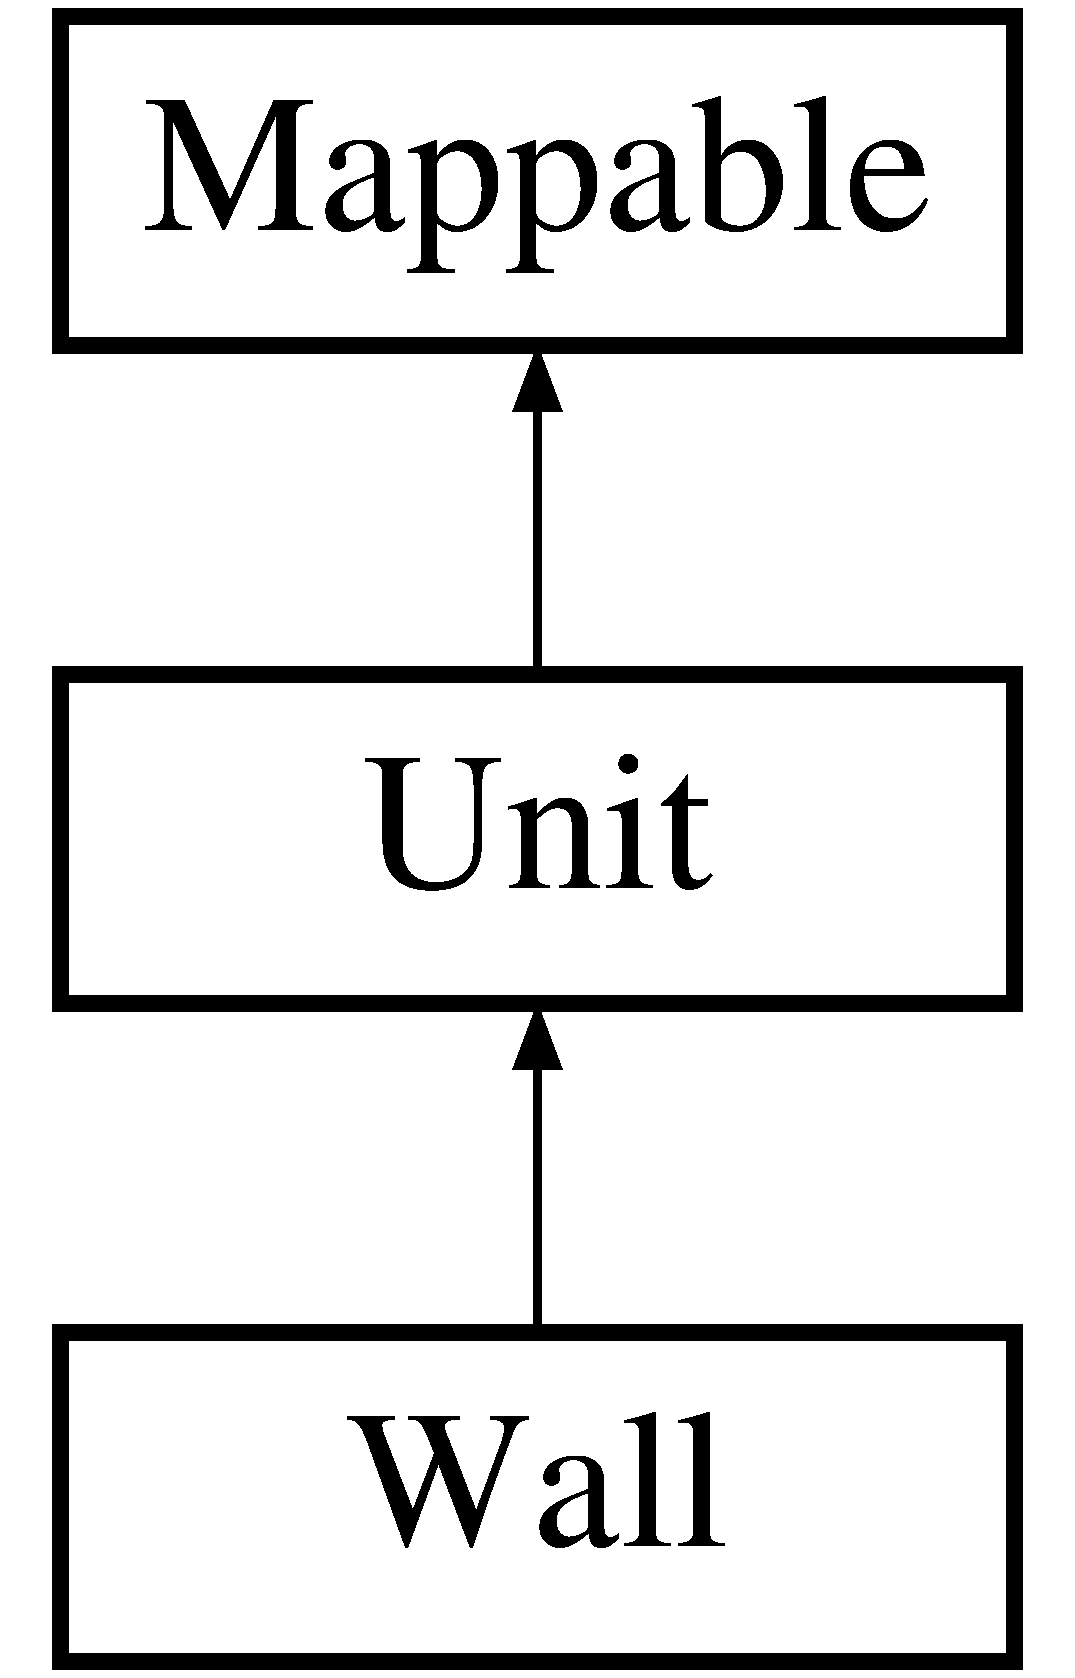
\includegraphics[height=3cm]{classWall}
\end{center}
\end{figure}
\subsection*{Public Member Functions}
\begin{DoxyCompactItemize}
\item 
\hypertarget{classWall_acbe8536be394e99f06a2d308c394d29d}{
{\bfseries Wall} (\hyperlink{struct__Wall}{\_\-Wall} $\ast$ptr=NULL)}
\label{classWall_acbe8536be394e99f06a2d308c394d29d}

\item 
\hypertarget{classWall_ad77bee6e20ca7c6979400fac6df22773}{
int \hyperlink{classWall_ad77bee6e20ca7c6979400fac6df22773}{id} ()}
\label{classWall_ad77bee6e20ca7c6979400fac6df22773}

\begin{DoxyCompactList}\small\item\em Unique Identifier. \item\end{DoxyCompactList}\item 
\hypertarget{classWall_af8bc6cd9cdc739eb990600b365db41bc}{
int \hyperlink{classWall_af8bc6cd9cdc739eb990600b365db41bc}{x} ()}
\label{classWall_af8bc6cd9cdc739eb990600b365db41bc}

\begin{DoxyCompactList}\small\item\em The X position of the top left corner of this object. X is horizontal. \item\end{DoxyCompactList}\item 
\hypertarget{classWall_aae93d1657e1fa8de7a04dda4882028c0}{
int \hyperlink{classWall_aae93d1657e1fa8de7a04dda4882028c0}{y} ()}
\label{classWall_aae93d1657e1fa8de7a04dda4882028c0}

\begin{DoxyCompactList}\small\item\em The Y position of the top left corner of this object. Y is vertical. \item\end{DoxyCompactList}\item 
\hypertarget{classWall_a7368d56ff031197c351d3eb3293e6cbc}{
int \hyperlink{classWall_a7368d56ff031197c351d3eb3293e6cbc}{owner} ()}
\label{classWall_a7368d56ff031197c351d3eb3293e6cbc}

\begin{DoxyCompactList}\small\item\em The owning player. \item\end{DoxyCompactList}\item 
\hypertarget{classWall_aa12d1a474f8960e3f6062af6e1605345}{
int \hyperlink{classWall_aa12d1a474f8960e3f6062af6e1605345}{health} ()}
\label{classWall_aa12d1a474f8960e3f6062af6e1605345}

\begin{DoxyCompactList}\small\item\em How much health this unit currently has. \item\end{DoxyCompactList}\item 
\hypertarget{classWall_ae5056228f0844e7a878ba730a11c0752}{
int \hyperlink{classWall_ae5056228f0844e7a878ba730a11c0752}{maxHealth} ()}
\label{classWall_ae5056228f0844e7a878ba730a11c0752}

\begin{DoxyCompactList}\small\item\em The maximum amount of health this unit can ever have. \item\end{DoxyCompactList}\item 
\hypertarget{classWall_a85e64eb011f3058640744958a3850c84}{
int \hyperlink{classWall_a85e64eb011f3058640744958a3850c84}{size} ()}
\label{classWall_a85e64eb011f3058640744958a3850c84}

\begin{DoxyCompactList}\small\item\em The length of one side of this \hyperlink{classUnit}{Unit}. \item\end{DoxyCompactList}\item 
\hypertarget{classWall_a714a3c6c90eb9abbfc01929c27c5bd7f}{
int \hyperlink{classWall_a714a3c6c90eb9abbfc01929c27c5bd7f}{talk} (std::string message)}
\label{classWall_a714a3c6c90eb9abbfc01929c27c5bd7f}

\begin{DoxyCompactList}\small\item\em Sends a message to be visualized when this unit is selected. \item\end{DoxyCompactList}\end{DoxyCompactItemize}
\subsection*{Friends}
\begin{DoxyCompactItemize}
\item 
\hypertarget{classWall_a0928c598df6be526ec9fadcc9a528d37}{
std::ostream \& {\bfseries operator$<$$<$} (std::ostream \&stream, \hyperlink{classWall}{Wall} ob)}
\label{classWall_a0928c598df6be526ec9fadcc9a528d37}

\end{DoxyCompactItemize}


\subsection{Detailed Description}
A pile of hard stuff that is in the way. 

The documentation for this class was generated from the following files:\begin{DoxyCompactItemize}
\item 
Wall.h\item 
Wall.cpp\end{DoxyCompactItemize}

\printindex
\end{document}
